%% If you have any problems using this template, please contact the author: %%
%% timhosgood@gmail.com. Updated for Statistics by SRH. Contact %%
%% ithelp@stats.ox.ac.uk if you have questions. %%
\documentclass{beamer}
\usepackage[utf8]{inputenc}
\usepackage{lmodern}
\usepackage{charter}
\usepackage{tikz}
\usepackage{graphicx}
\usepackage{amsmath}
\usepackage{amssymb}
\usepackage[round]{natbib}
\usepackage{bibentry}
\usepackage{bm}
\newcommand{\ud}{\,\mathrm{d}}
\newcommand{\vx}{\mathbf{x}}
\usetheme{Copenhagen}
\usecolortheme{rose}
\setbeamertemplate{navigation symbols}{}

%% Title slide formatting %%
\pgfdeclareimage[height=0.9cm]{uoblogo}{images/UoB-logo-colour}
\pgfdeclareimage[height=1.2cm]{GMlogo}{images/GM-logo}
\pgfdeclareimage[height=0.7cm]{GMteam}{images/GMteam}

%\pgfdeclareimage[width=3.3cm]{manifestation}{images/G_Mani.png}
\definecolor{GMred}{RGB}{150,10,10}
\definecolor{GMblue}{RGB}{10,100,220}
\definecolor{GMgrey}{RGB}{64,64,64}
\setbeamerfont{title}{size=\huge}
\setbeamerfont{author}{size=\normalsize}
\setbeamerfont{subtitle}{size=\small}

\setbeamertemplate{title page}{
    \begin{picture}(0,0)       
        \put(30,-85){%
            \begin{minipage}[b][4.5cm][t]{0.8\textwidth}
            \begin{center}
                \color{GMred}\usebeamerfont{title}
                    {\inserttitle\\[0.5cm]}
                    \color{GMblue}
                \usebeamerfont{author}               
                    {\insertauthor\\[0.3cm]}
                \usebeamerfont{subtitle}                                   
                    {\insertinstitute\\[0.3cm]}
                    \color{black}
                    {\insertdate}
                    \end{center}
            \end{minipage}        
        }
        \put(-10, 70){%
        	\pgfuseimage{uoblogo}
        	}
        	\put(220, 65){%
        	\pgfuseimage{GMlogo}
        	}
        	  \put(-17, 60){%
             \rule{340pt}{0.4pt}
        }	
    \end{picture}
}

%% General slide formatting %%
\setbeamertemplate{headline}
{%
    \begin{picture}(0,0)
        \put(290,-24){%
            \scalebox{0.65}{\pgfuseimage{uoblogo}}
        }
         \put(287,-48){%
            \scalebox{0.65}{\pgfuseimage{GMlogo}}
        }
        \put(12,-50){%
             \rule{340pt}{0.4pt}
         }
    \end{picture}
}

\setbeamerfont{frametitle}{size=\LARGE}
\setbeamerfont{framesubtitle}{size=\large}
\setbeamertemplate{frametitle}
{%

    \begin{picture}(0,0)
        \put(-12,-12){%
			\color{GMred}
			\usebeamerfont{frametitle}{\insertframetitle}
        }
        \put(-10,-30){%
			\color{GMblue}
			\usebeamerfont{framesubtitle}{\insertframesubtitle}
        }            
    \end{picture}
}

\setbeamertemplate{footline}
{%
    \begin{picture}(0,0)
        \put(12,27){%
            \rule{340pt}{0.4pt}
        }
        \put(15,14){%
            \color{GMgrey}\insertshortauthor
        }
        \put(175,14){%
            \color{GMgrey}\insertpagenumber
        }
        \put(280, 6){%
        	\pgfuseimage{GMteam}
        	}
    \end{picture}%
}
% Date customisation
\renewcommand{\today}{\number\day\space \ifcase\month\or
  January\or February\or March\or April\or May\or June\or
  July\or August\or September\or October\or November\or December\fi
   \space\number\year}

%% Information (author, title, etc.) %%
\color{GMred}
\title[BHM for GIA and global sea level rise]{Bayesian estimation of global glacial isostatic adjustment for sea level rise re-evaluation} % short title for footer
\author%
[Z. Sha et. al]{Zhe Sha\textsuperscript{1},  Maike Schumancher\textsuperscript{1},  \\ 
 Jonathan Rougier\textsuperscript{2} and Jonathan Bamber\textsuperscript{1}
}
\institute%
{%
    \textsuperscript{1}School of Geographical Sciences,\textsuperscript{2}School of Mathematics\\
    University of Bristol
}

\date{26\space July \space 2017}

%---------------------------------------------------------------------------------------%
%---------------------------------------------------------------------------------------%

\begin{document}

%-----------------Title Page------------------%
\begin{frame}[plain]
      \titlepage
\end{frame}
% Return default slide background colour to white.
\setbeamercolor{background canvas}{bg=white}

%------------Section: Motivation--------------%
\section{Motivation}
%----------- slide --------------------------------------------------%
\begin{frame}
\frametitle{GlobalMass}
\framesubtitle{A 5-year project for global sea level rise re-evaluation}


\emph{\textbf{GlobalMass}}
\begin{itemize}
\item combine satellite and in-situ data related to different aspects of the sea level budget,
\item attribute global sea level rise to its component parts.
\end{itemize}


\begin{center}

\includegraphics[width = 0.18\textwidth, clip]{images/EUflag}
\hspace{2cm}

\includegraphics[width = 0.15\textwidth, clip]{images/ERClogo}
\end{center}
 
    \footnotesize{Funded by the European Research Council (ERC) under the European Union's Horizon 2020 research and innovation programme under grant agreement No 69418.}




\end{frame}
%----------- slide --------------------------------------------------%
\begin{frame}
\frametitle{Global sea level rise re-evaluation}
\begin{block}{The sea level budget \emph{enigma}}
\begin{align*}
&\Delta \mbox{sea level} (t) \hspace{0.1cm}= \hspace{0.1cm} \Delta\mbox{barystatic}(t) \hspace{0.2cm} + \hspace{0.2cm} \Delta\mbox{steric}(t) \hspace{0.5cm}+ \hspace{0.5cm} \mbox{GIA}\\
&\color{red}\hspace{3.3cm} \mbox{mass} \hspace{2cm}\mbox{density} \hspace{1.2cm} \mbox{ocean basins}
\end{align*}

- GIA: glacial isostatic adjustment

- inconsistencies between the discipline-specific estimates
\end{block}
\begin{block}{GlobalMass Aims}
\begin{itemize}
\item simultaneous global estimates of all the components
\item close the sea level budget
\end{itemize}
\end{block}

%----------- slide --------------------------------------------------%
\end{frame}

\begin{frame}{The Bayesian hierarchical model}
\framesubtitle{Framework concept \citep{AZM2015}}
\vspace{0.5cm}
\centering
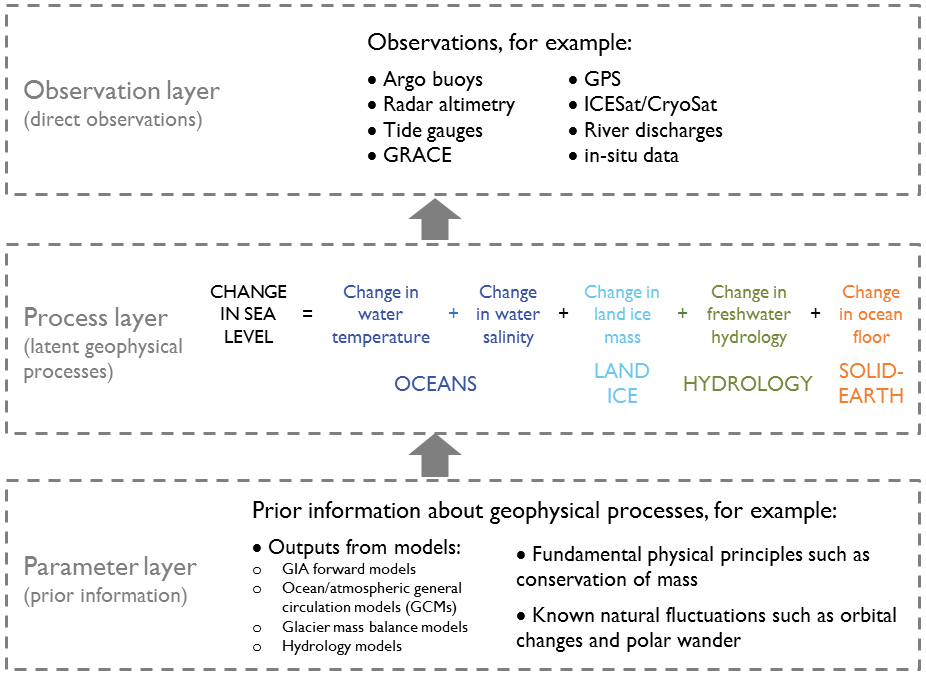
\includegraphics[height =0.7\textheight]{images/GMconcept-simplified}

\end{frame}

%----------- slide --------------------------------------------------%
\section{modeling the GIA process}
\begin{frame}
\frametitle{First step -- modelling GIA}
\framesubtitle{What is GIA?}


\begin{minipage}[c]{0.4\textwidth}
\includegraphics[width = \textwidth]{images/gia}

\tiny{Figure courtesy of the Canadian Geodetic Survey, Natural Resources Canada.}
\end{minipage}%
\hfill
\begin{minipage}[c]{0.55\textwidth}
\textbf{GIA - glacial isostatic adjustment}
\begin{itemize}
\item  vertical displacement of the Earth's crust once burdened by ice-age glaciers (\textcolor{red}{$\sim$20,000 yrs ago})
\item  constant over the time scale of this study (\textcolor{red}{1981-2020})
\item Regional discrepancies in estimates from physical models, e.g. ICE-6G \citep{Peltier}
\end{itemize}
\end{minipage}


\end{frame}


%----------- slide --------------------------------------------------%
\begin{frame}{The GIA process}

\vspace{0.5cm}
\begin{minipage}[c]{0.4\textwidth}
\textcolor{blue}{true GIA process} 

$\bm{Y}: \mathbb{S}^2 \mapsto \mathbb{R}$

\vspace{0.5cm}
\textcolor{blue}{prior mean trend}

$\bm{\mu}: \mathbb{S}^2 \mapsto \mathbb{R}$
\end{minipage}%
\begin{minipage}[c]{0.55\textwidth}
\centering
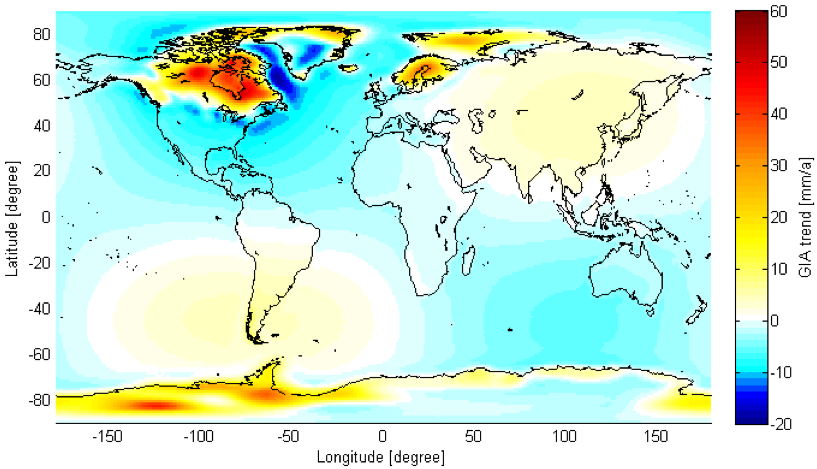
\includegraphics[width = \textwidth, clip]{images/ice6g}

\tiny{GIA estimates from a ICE-6G model.}
\end{minipage}

\vspace{0.3cm}
After de-trend, the residuals become stationary and assume
\begin{align}\label{eq:GIAresid}
 \bm{X}: = \bm{Y} - \bm{\mu} \sim \mathcal{GP}(\bm{0}, \kappa(\bm{\theta}))
\end{align}
$\kappa(\bm{\theta})$ -- Mat{\'e}rn covariance function with parameter $\bm{\theta} = (\rho, \sigma^2)$ for the length-scale and variance.

\end{frame}

%----------- slide --------------------------------------------------%
\begin{frame}{The GPS observations}
\framesubtitle{Vertical movement in the Earth's surface}
\vspace{0.3cm}
GPS times series signals at Station $i$,
\begin{itemize}
\item[-] an uplift rate $Z_i$ (mm/yr)
\item[-] a measurement error  $\varepsilon_i \sim \mathcal{N}(0, e_i^2)$
\item[-] $e_i = \mbox{s.d.}(Z_i)$ estimated from the time series.
\end{itemize} 

\begin{minipage}[c]{0.4\textwidth}
\centering
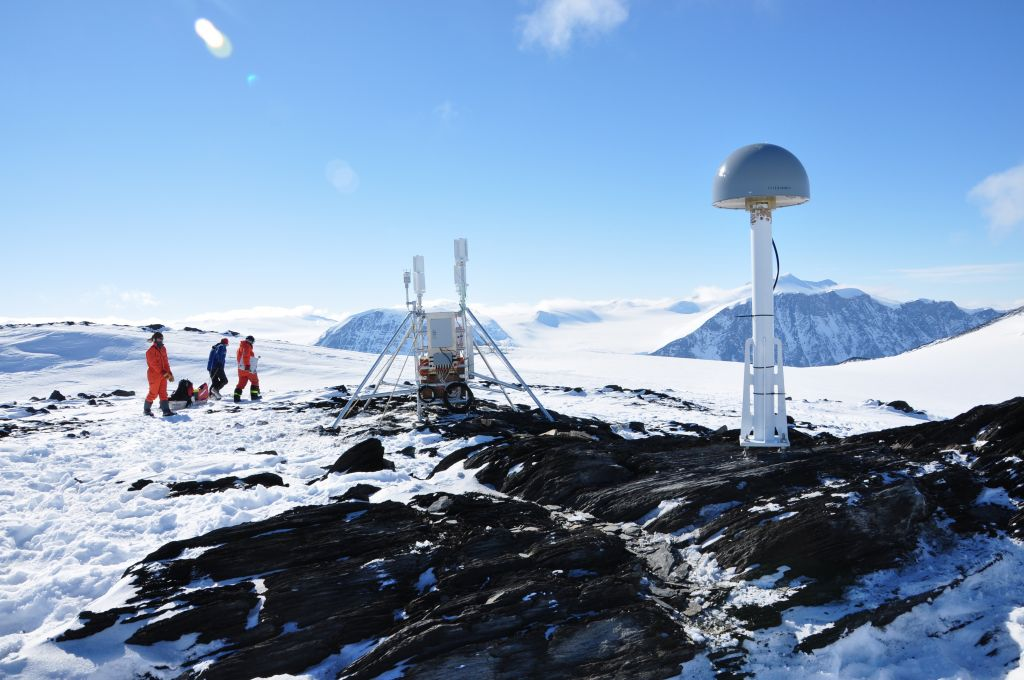
\includegraphics[width=0.8\textwidth]{images/GPSstation}

\tiny{A GPS station in Antarctic.}
\end{minipage}%
\hfill
\begin{minipage}[c]{0.6\textwidth}
\centering
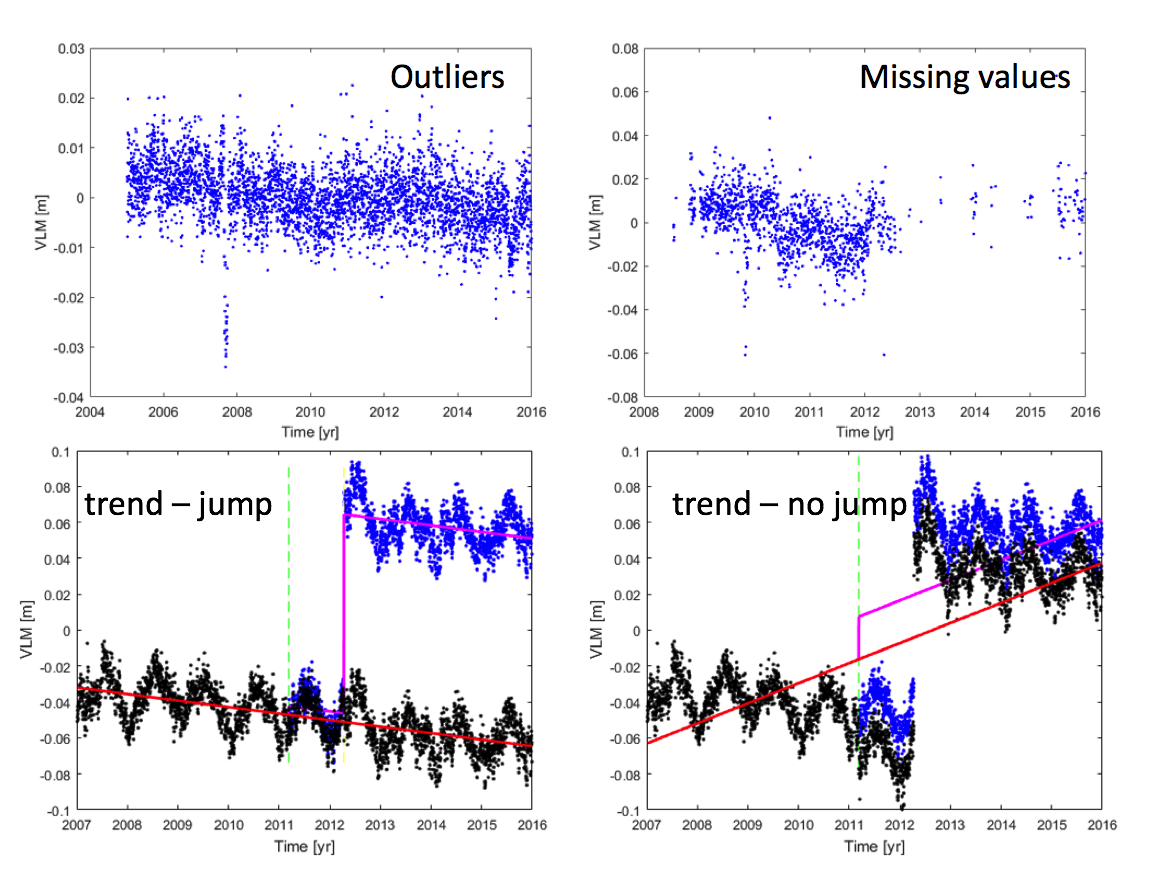
\includegraphics[width=0.8\textwidth]{images/GPSts}
\end{minipage}


\end{frame}

%----------- slide --------------------------------------------------%
\begin{frame}{Forward modelling}
\framesubtitle{From process to observations}

\begin{minipage}[c]{0.48\textwidth}
\begin{center}
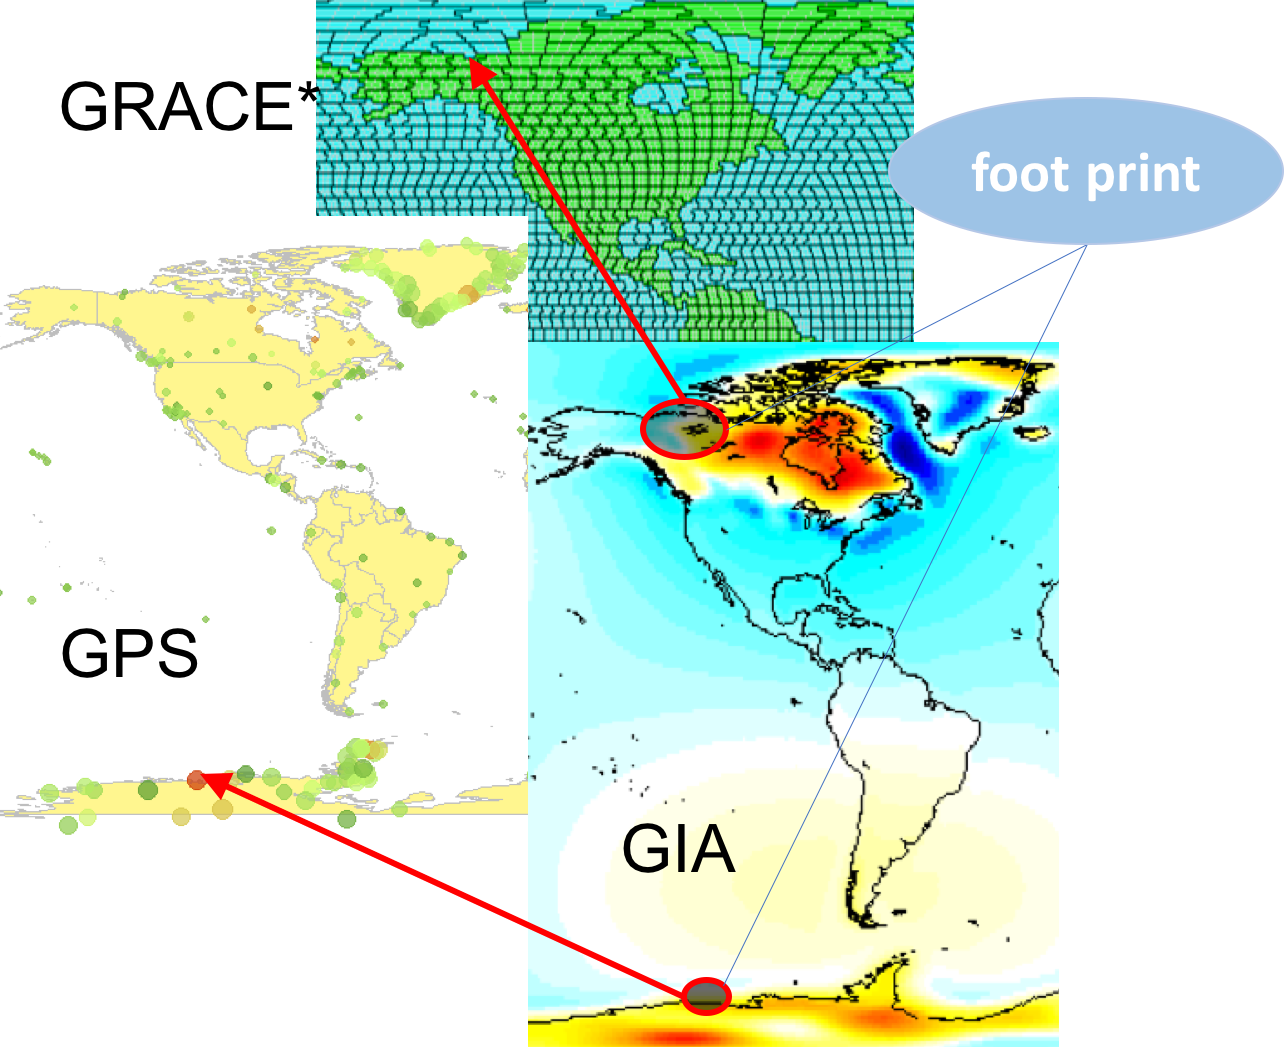
\includegraphics[width = \textwidth]{images/footprint}
\end{center}
\tiny{*GRACE: the Gravity Recovery And Climate Experiment satellites}

\end{minipage}%
\hfill
\begin{minipage}[c]{0.5\textwidth}
$\bm{\mathcal{A}_i}$ maps the latent process over the appropriate spatial \emph{\textbf{foot print}} to the $i^{th}$ observation,
\begin{align}\label{eq:GPSi}
Z_i = \bm{\mathcal{A}}_i\bm{Y} + \varepsilon_i, 
\end{align} 

 $\bm{\mathcal{A}_i}$ is usually a linear operator 
 \begin{itemize}
 \item point $\to$ point
 \item area $\to$ point
 \item area $\to$ area
 \end{itemize}
\end{minipage}

\end{frame}

%----------- slide --------------------------------------------------%
\begin{frame}{The BHM for GIA}
\vspace{0.3cm}
Denote by $\bm{\mathcal{A}}^T = \left[
 \bm{\mathcal{A}}_1^T, \cdots,\bm{\mathcal{A}}_N^T \right]$,
then we can have the vector form for equation \eqref{eq:GPSi}
\begin{align}\label{eq:GPS}
\bm{Z} = \bm{\mathcal{A}}\bm{Y} + \bm{\varepsilon} 
\end{align}
\begin{block}{Bayesian hierarchical model for GIA}
Combine the observation equation \eqref{eq:GPS} and the process equation \eqref{eq:GIAresid}
\begin{align}\label{eq:BHM}
\left\{ \begin{array}{l}
\bm{\tilde{Z}} = \bm{\mathcal{A}}\bm{X} + \bm{\varepsilon}, \; 
\bm{\varepsilon} \sim \mathcal{N} (\bm{0}, \mbox{diag}(e_1^2, e_2^2, \dots, e_N^2)) \\
\bm{X} \sim \mathcal{GP}(\bm{0}, \kappa(\bm{\theta})) \\
\bm{\theta} \sim \bm{\pi}(\bm{\theta})
\end{array} \right.
\end{align}
\end{block}

\end{frame}

\begin{frame}{Predicting GIA}
\framesubtitle{The predictive distribution of the latent process}
\begin{block}{Predictive Distribution of GIA}
The prediction is based on the posterior marginal distribution of the latent process 
\begin{align}
\bm{\pi}(\bm{X} | \bm{\tilde{Z}})= \int_{\bm{\Theta}} \bm{\pi}(\bm{X}, \bm{\theta}| \bm{\tilde{Z}})\ud \bm{\theta}
\end{align}

\textcolor{red}{-- Integrating the uncertainty of the parameters.}
\end{block}

Other choices include the ``plug-in'' predictive distribution $\bm{\pi}_{p}(\bm{X} | \bm{\tilde{Z}}) = \bm{\pi}_{p}(\bm{X} | \bm{\tilde{Z}}, \bm{\hat{\theta}})$, where $\bm{\hat{\theta}}$ are the estimated values of the parameters, e.g. posterior mean or mode.
\end{frame}

\begin{frame}{Predicting GIA}
\framesubtitle{Point-wise prediction of the latent process}
\begin{block}{Point-wise predicted mean and uncertainty}
For point-wise update at $X_i$ on a fine grid, we use 
\begin{align*}
&\mbox{predicted mean:} X_i^* = \mathbb{E}(X_i| \bm{\tilde{Z}}) \\
&\mbox{predicted uncertainty:} u_i^* = \mbox{s.d.}(X_i| \bm{\tilde{Z}})
\end{align*}
where $\bm{\pi}(X_i | \bm{\tilde{Z}}) = \int_{\bm{\mathcal{X}_{-i}}} \bm{\pi}(\bm{X} | \bm{\tilde{Z}}) \ud \bm{X_{-i}}$.

\end{block}
When using the ``plug-in'' predictive distribution, $\bm{\pi}_{p}(X_i | \bm{\tilde{Z}})$ is Gaussian and the Bayesian update can be written in closed form.
\end{frame}




%----------- Section --------------------------------------------------%
\section{The SPDE Approach}
\begin{frame}{The GMRF approximation}
\begin{itemize}
\item Bayesian update of the GP on a grid of $m$ points scales as $\mathcal{O}(m^3)$, $m \sim 10^5$ for a $1^\circ $ global grid.
\item Gaussian Markov random field (GMRF) with sparse precision matrix has a much better scaling property.
\end{itemize}

\begin{block}{The SPDE approach \citep{Lindgren2011}} 

Denote by $\bm{\mathrm{x}}$ the GMRF approximation of $\bm{X}$ on a triangulation of $m$ vertices with basis functions $\{ \bm{\phi}_i \}_{i \in \mathbb{N}}$, then  $s \in \mathbb{S}^2$
\begin{align}
\bm{X}(s) \approx \bm{\phi}_i(s)^T\bm{\mathrm{x}}
\end{align}
For a grid $\bm{S} \subset \mathbb{S}$ of locations, we find the weight matrix $\bm{C}$ and write $\bm{X}(\bm{S}) \approx \bm{C}\bm{\mathrm{x}}$.
\end{block}
\end{frame}

\begin{frame}{The GMRF approximation}
Now the BHM in equation \eqref{eq:BHM} becomes
\begin{align}\label{eq:BHM_gmrf}
\left\{ \begin{array}{l}
\bm{\tilde{Z}} = \bm{\mathcal{A}}\bm{C}\bm{\mathrm{x}} + \bm{\varepsilon}, \; 
\bm{\varepsilon} \sim \mathcal{N} (\bm{0}, \mbox{diag}(e_1^2, e_2^2, \dots, e_N^2)) \\
\bm{\mathrm{x}} \sim \mathcal{N}(\bm{0}, \bm{Q}^{-1}(\bm{\theta})) \\
\bm{\theta} \sim \bm{\pi}(\bm{\theta})
\end{array} \right.
\end{align}
$\bm{\mathrm{x}} $ is GMRF approximation defined by the precision matrix $\bm{Q}$.

\end{frame}

%----------- slide --------------------------------------------------%
\begin{frame}{Choosing the mesh on a sphere}
\vspace{0.7cm}
\begin{minipage}[c]{0.4\textwidth}
\centering
\footnotesize{semi-regular mesh}

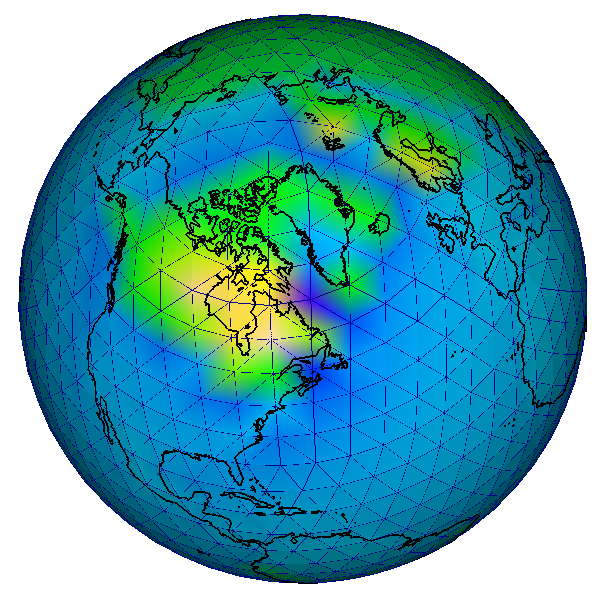
\includegraphics[width=0.7\textwidth]{images/GIA_mesh1}
\vspace{0.5cm}

\footnotesize{irregular mesh}

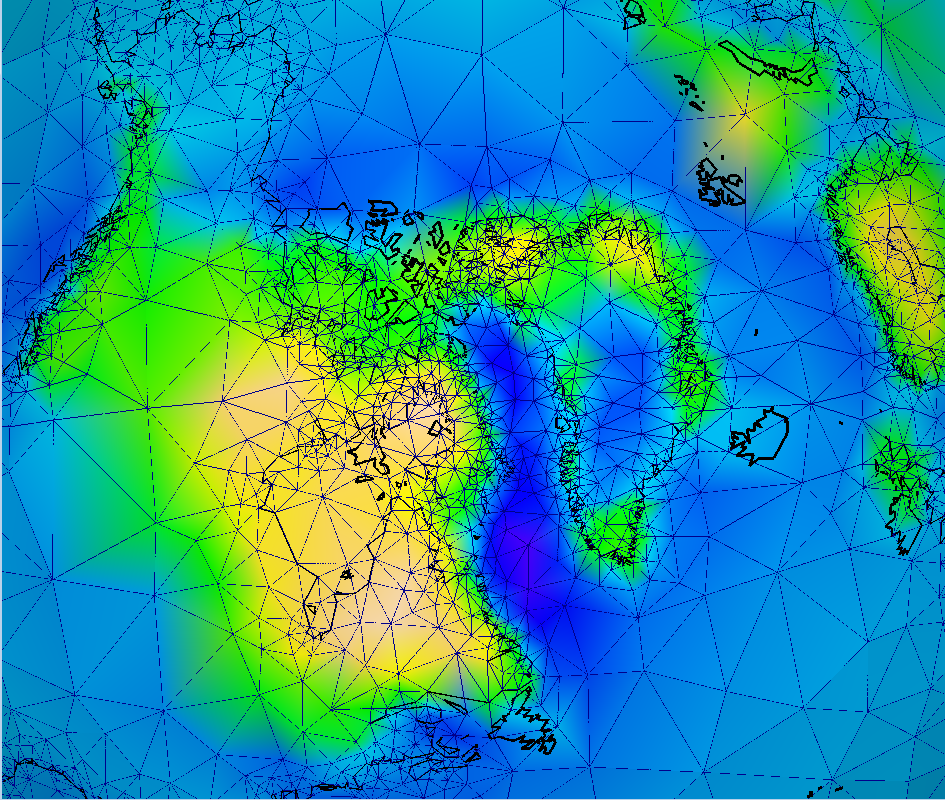
\includegraphics[width=0.6\textwidth]{images/GIA_mesh2}
\end{minipage}%
\hfill
\begin{minipage}[c]{0.6\textwidth}
\centering
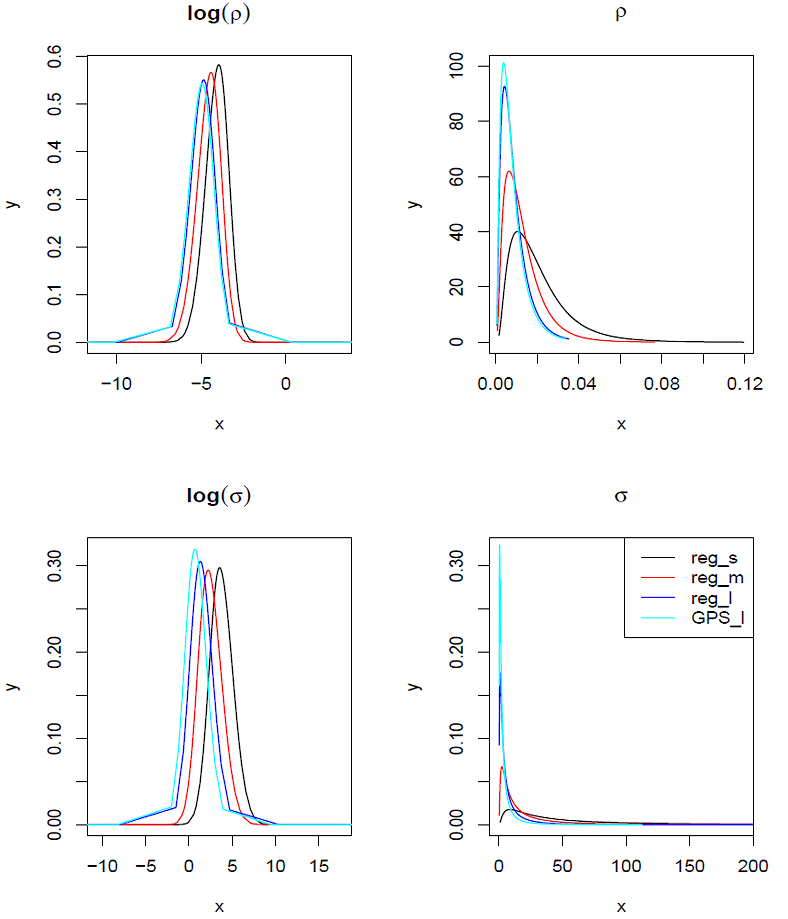
\includegraphics[width=0.8\textwidth]{images/mesh_pars}

\footnotesize{Parameter estimation using different meshes.}
\end{minipage}%

\end{frame}

%----------- Section --------------------------------------------------%
\begin{frame}{Mesh effect}
\framesubtitle{The predicted uncertainties using regular mesh}

\vspace{0.7cm}
\centering
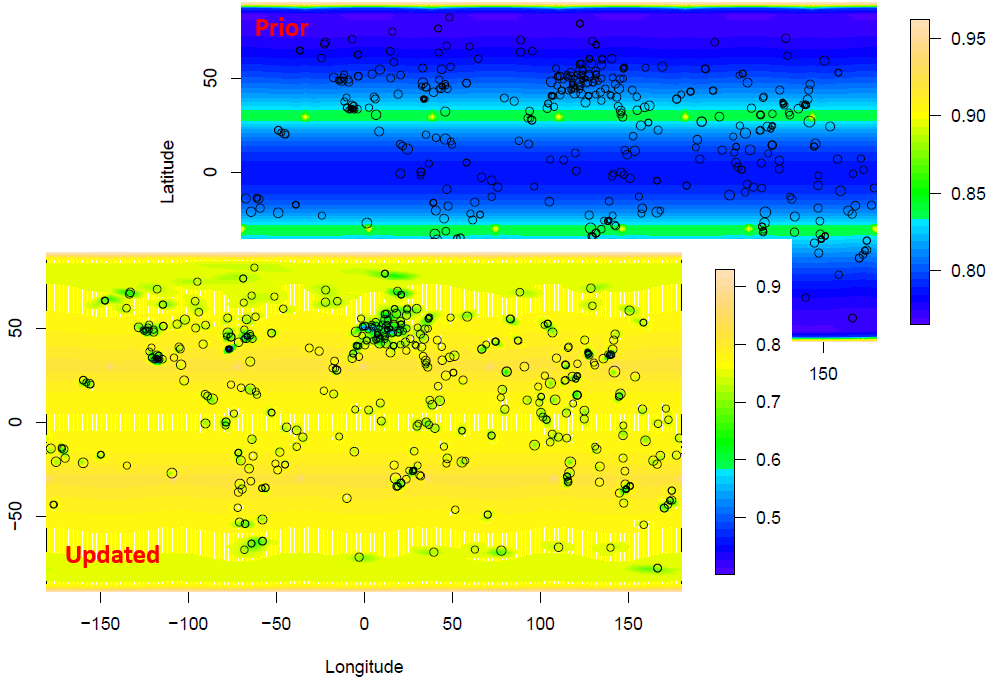
\includegraphics[width = 0.9\textwidth]{images/reg_var}
\end{frame}

%----------- Section --------------------------------------------------%
\begin{frame}{Mesh effect}
\framesubtitle{The predicted uncertainties using irregular mesh}

\vspace{0.7cm}
\centering
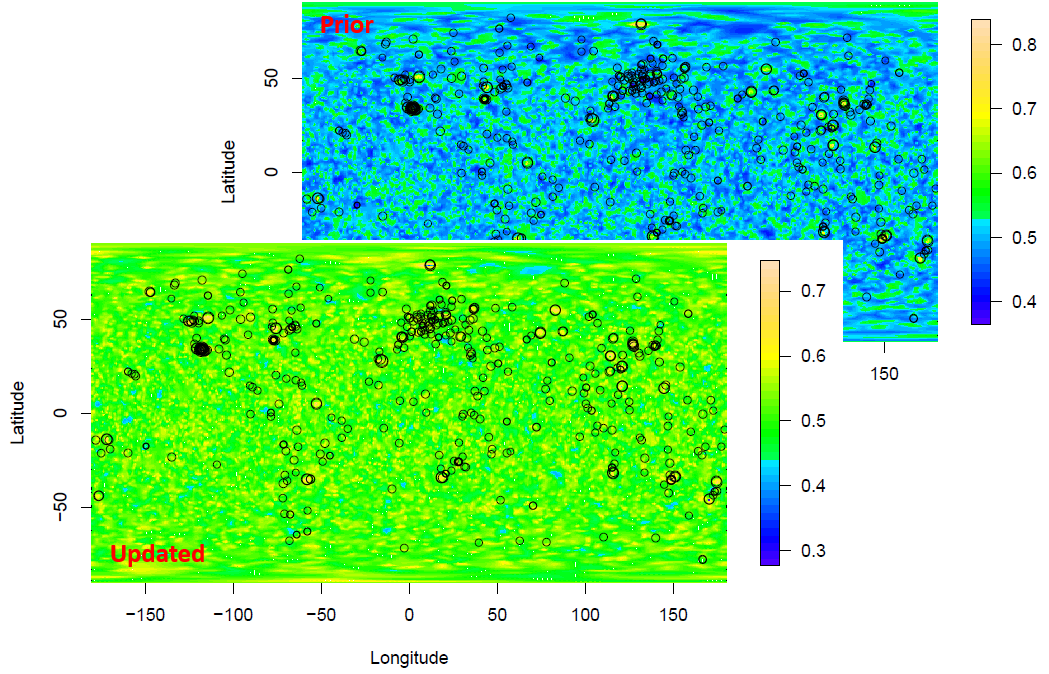
\includegraphics[width = 0.9\textwidth]{images/irreg_var}
\end{frame}

%----------- Section --------------------------------------------------%
\section{First result for GIA}
\begin{frame}{First solution for GIA}
\vspace{0.5cm}
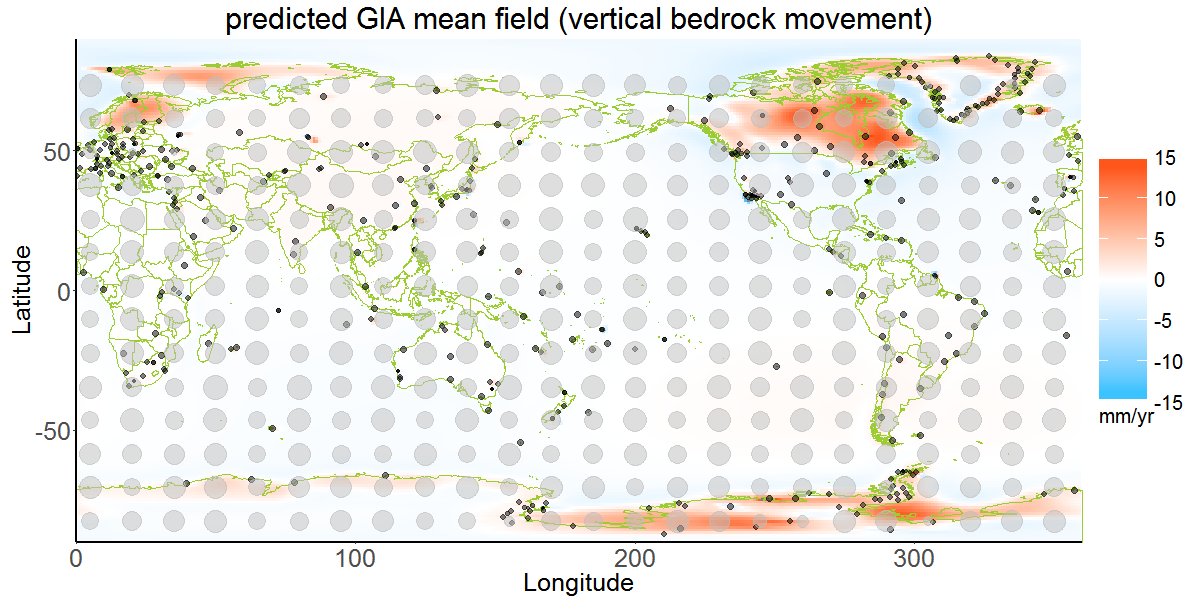
\includegraphics[width = 1.05\textwidth]{images/GIA_map}

\centering
\footnotesize{GIA disc size (grey) proportional to predicted uncertainty}
\end{frame}

%----------- Section --------------------------------------------------%
\section{Conclusion}
\begin{frame}{Conclusions and outlook}

\begin{itemize}
\item Testing the statistical framework for the GIA.
\item Requiring improved mesh.
\begin{itemize}
\item Adaptive -- fast computation
\item Regular -- stable approximation
\end{itemize}
\item Improving GPS data quality.
\item Extending to the full system.
\end{itemize}


\end{frame}

%----------- slide --------------------------------------------------%
\begin{frame}{References}
\bibliographystyle{apalike}
\small{\bibliography{references}}
\end{frame}


\begin{frame}{Questions}
\centering
\Huge
Thank you!
\end{frame}


\end{document}